\documentclass[11pt]{article}
\usepackage[margin=1in]{geometry}          
\usepackage{amsthm, amsmath, amssymb}
\usepackage{setspace}\onehalfspacing
\usepackage[loose,nice]{units} 
\usepackage[document]{ragged2e}
\usepackage{caption}
\newcommand{\source}[1]{\caption*{Source: {#1}} }
\usepackage{tikz}
\usepackage{cancel}
\usepackage{textcomp}
\usepackage{empheq}
\newcommand*\widefbox[1]{\fbox{\hspace{2em}#1\hspace{2em}}}
\usepackage{pgfplots}
\usetikzlibrary{patterns}
\usepackage[utf8]{inputenc}
\usepackage{graphicx}
\usepackage{subfig}
\newcommand\multi{1.3}
\usepackage{geometry}

\renewcommand\floatpagefraction{.9}
\renewcommand\topfraction{.9}
\renewcommand\bottomfraction{.9}
\renewcommand\textfraction{.1}   
\setcounter{totalnumber}{50}
\setcounter{topnumber}{50}
\setcounter{bottomnumber}{50}
\setlength{\tabcolsep}{1.3pt}
\renewcommand{\arraystretch}{0.5}


%%%%%%% NOTES %%%%%%%
%Include details on how to extend every project
%Include limitations of methods
%Talk about dimensions of all simulations
%Work out how many terms is a second etc in simulation
%(The general time complexity of n body equations is o($n^2$))
%total list 10,000 points over 20s





%%%%%%%%%%%%%%%%%%%FIXING!!!!!!%%%%%%%%%%%%%%
% ECCENTRICITY VECTOR FOR BOTH
% POTENETIAL ENERGY GRAPH

 %PAGE 1
\title{Computational Physics: \newline
Complex Orbital Dynamics}
\date{2023}

\begin{document}
\maketitle
\bigskip
\bigskip
\bigskip
\bigskip
\bigskip
\bigskip


%%% ----------- Rewrite so not exactly the same as the abstract -----------------------------
\centering
\parbox{350pt}{
The solutions and simulations of the orbital motion of bodies under the influence of gravity is an important problem which this report will study using a variety of computational techniques. We will apply some of these techniques to more realistic problems as well as idealised problems for objects of the same mass, looking at their stability, accuracy and conservation of energy and angular momentum.
}



 
\newpage

% --------------------------------------------------SECTION 1---------------------------------------------------------------------------------------------------------------------
\newgeometry{left=2cm,bottom=2cm,top=2cm,right=2cm}
\section{Background}
\raggedright
We will be looking for stable solutions of orbits for 2 to 8 bodies under the regime of classical Newtonian gravity, however some solutions considered can theoretically be extended to any number of bodies. 

\bigskip
The computational techniques used in this project are:
\begin{itemize}
\item Euler's method
\item Velocity Verlet integration
\item  Runge Kutta 4th order (using SciPy integrate.solve\_ivp with method 'RK45' and relative tolerance set to 1e-6)
\end{itemize}

\bigskip

The orbit types we will be considering are:
\begin{itemize}
\item 2 bodies with central mass fixed
\item 2 bodies with central mass allowed to move
\item 3 bodies in a Sun-Earth-Moon like regime
\item N bodies in a circular orbit
\item N bodies in a linear chain
\item Complex choreographies of 3 bodies
\end{itemize}

\bigskip
For all different types of orbit we will consider their stability and sensitivity to initial conditions. We will be setting the gravitational constant $G$ = 1, this is to simplify differential equations and also gives a smaller disparity in orders of magnitude between numbers in the calculations, which can lead to faster convergence of numerical methods \cite{NbodyScipy}. Doing this does not affect the comparisons between methods and orbits and just acts as a non-dimensionalization rescaling of the problem.


% --------------------------------------------------SECTION 2---------------------------------------------------------------------------------------------------------------------
\centering
\section{Newtonian Gravity and associated differential equations}
\raggedright

For this project we will be using newtonian gravity, this is a classical representation of orbits and neglects relativistic effects, however is still a useful approximation to simulate the orbits we are interested in, making the computational task easier and keeping fairly accurate. We are also only considering circular orbits in the first 5 sections rather than the more realistic elliptical orbits.
\bigskip

In Newtonian gravity, the force on a body, 1, due to a body, 2, is given by the equation:

$$
\textbf{F}_{12} = \frac{G m_1 m_2}{|\textbf{r}_{21}|^3} \textbf{r}_{21}
$$

\smallskip

Due to Newton's third law, $\textbf{F}_{21} = - \textbf{F}_{12}$ and using Newton's second law we can obtain the equation of motion for object 1 in this system in the form of the differential equation:

$$ \textbf{F} = m_1 \textbf{a}_1 = \frac{G m_1 m_2}{|\textbf{r}_{21}|^3} \textbf{r}_{21}$$

$$
\frac{d^2\textbf{r}_1}{dt^2} =  G m_2 \frac{\textbf{r}_{21}}{|\textbf{r}_{21}|^3}
$$

This differential equation can easily be extended to N bodies by just adding their forces:

$$
\frac{d^2\textbf{r}_1}{dt^2} =  G m_2 \frac{\textbf{r}_{21}}{|\textbf{r}_{21}|^3} + G m_3 \frac{\textbf{r}_{31}}{|\textbf{r}_{31}|^3} + \cdots + G m_N \frac{\textbf{r}_{N1}}{|\textbf{r}_{N1}|^3}
$$
\bigskip

In some sections we will also be calculating the kinetic energy (KE), potential energy (PE) and angular momentum (L) which are given by:

$$
KE = \frac{1}{2} m \textbf{v}^2
$$
$$
PE = - \frac{G M m}{r}
$$
$$
L = m (v \times r)
$$

% --------------------------------------------------SECTION 3---------------------------------------------------------------------------------------------------------------------
\centering
\section{Euler's Method}
\raggedright
\subsection{Method and equations}

Euler's method for solving differential equations is a simple approach and therefore easy to implement, however is also prone to instabilities and inaccuracies which I will discuss more below. 
\bigskip

The formula for Euler's method is obtained from the definition of a finite differential:
\begin{equation}
\label{EulerDefinition1}
\frac{dy}{dt} \simeq \frac{y(t+\Delta t) - y(t)}{\Delta t} 
\end{equation}
\begin{equation}
\label{EulerDefinition2}
\Rightarrow y(t + \Delta t) = y(t) + \Delta t \frac{dy(t)}{dt}
\end{equation}

Because we have a 2nd order differential equation for our equations of motion, we will need to calculate \textbf{r} and $\frac{d\textbf{r}}{dt}$ (velocity) at each time step. These are then given by the equations:

$$
\textbf{r}(t+\Delta t)= \textbf{r}(t) + \Delta t \frac{d \textbf{r}(t)}{dt} 
$$
$$
\textbf{v}(t+\Delta t)= \textbf{v}(t) + \Delta t \frac{d \textbf{v}(t)}{dt} 
$$
\bigskip

With $\frac{d \textbf{r}(t)}{dt} = \textbf{v}(t)$ and  $\frac{d \textbf{v}(t)}{dt} = \frac{d^2\textbf{r}}{dt^2} = \textbf{a}(t)$


\subsection{Implementation}

\begin{figure}[ht]
\centerline{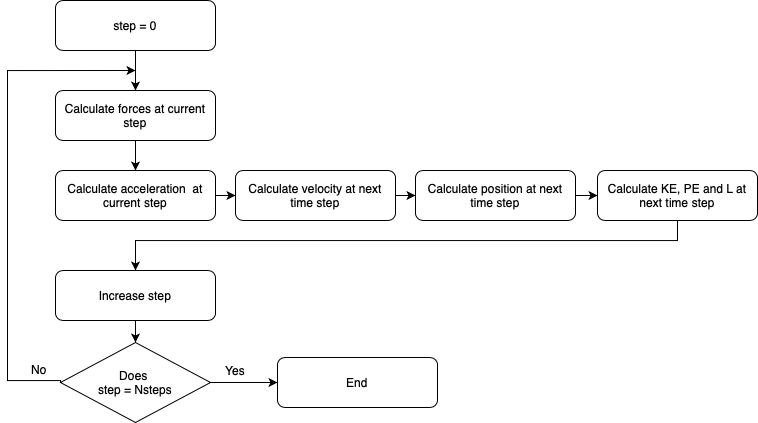
\includegraphics[scale=0.56]{Pictures/EulerMethod.png}}
\caption{A flow chart representing the steps in the Euler method with Nsteps the maximum number of steps the cycle is run for.}
\label{spectrum_ripples}
\end{figure}

\subsection{Initial conditions}

We will be testing Euler's method by simulating the orbit of a planet around a fixed central mass. We will be using a large difference in the sizes of the mass so that the approximation that the central mass does not move is not too unreasonable. To do this, we set the position of body 2 to be the origin and do not update its position. We will give this object a mass of 1. 
We set another object at (1, 0) which we give a mass of 0.0001 and will orbit around the central mass. To work out the initial conditions to obtain a circular orbit for this scenario we can use circular motion equations:

$$
\frac{m_1 v^2}{r} = \frac{G m_1 m_2}{r^2}
$$
And with $G = m_2 = r = 1$ this reduces to:

$$ v^2 = 1 \implies v_y = \pm 1$$
Choosing $v = +1$ so that the object rotates anti-clockwise.

\newpage
\subsection{Plots of the Euler simulation}
\begin{figure}[!ht]
\centerline{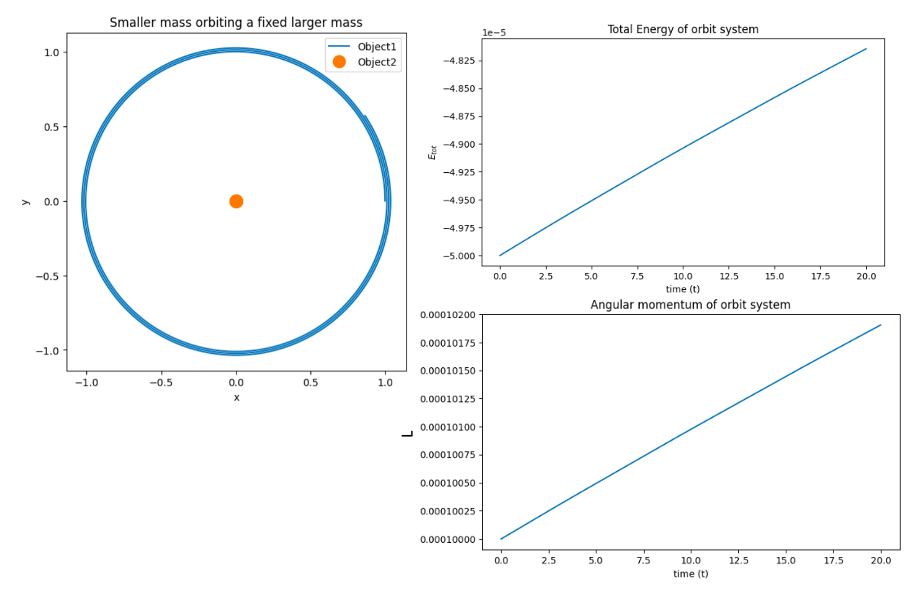
\includegraphics[scale=0.5]{Pictures/EulerGraph.png}}
\caption{Plots from Euler method simulation}
\label{EulerGraph}
\end{figure}



\subsection{Analysis of the graphs}

It is clear to see from this simulation that the Euler method is not particularly accurate as we can see that the outer mass spirals outwards. From looking at the graphs of the total energy and angular momentum we can see these increase linearly with time, changing by 3.5\% and 0.2\% respectively. While this may seem like a small deviation, when simulating more complex dynamics this error can quickly compound to create larger errors and distinctly change the look of the orbit.

\subsection{Euler inaccuracies}

Doing some mathematical analysis of Euler's method, we can see why these errors occur. From the original definition of the derivative (eq \ref{EulerDefinition1}) we can see that this finite differential only holds in the limit that $\Delta t \rightarrow 0$ which of course cannot be simulated on a computer. 
\smallskip
We should instead write eq \ref{EulerDefinition2} as a Taylor expansion:
\begin{equation}
y(t + \Delta t) = y(t) + \Delta t \frac{dy(t)}{dt} + \frac{(\Delta t)^2}{2!} \frac{d^2y}{dt^2} + O(\Delta t^3)
\label{Taylor}
\end{equation}

Which gives a leading term in the error of$ (\Delta t)^2$, however this is just the error in a single step, the global error is the sum of the errors for the number of steps required to reach $x$ from $x_0$: $N=\frac{t-t_0}{ \Delta t}$, so that the global error (N times the error in each step) will be of order $\Delta t$ \cite{Briefing}.

% --------------------------------------------------SECTION 4---------------------------------------------------------------------------------------------------------------------
\centering
\section{The Velocity Verlet Method}
\raggedright




We have now seen that the Euler method is not very accurate and has large errors, so we will now look at a different, more accurate solver called Velocity Verlet.

Velocity Verlet is a time reversible method, which is useful for solving newtonian equations of motion which are also meant to be time reversible, meaning energy and angular momentum should be conserved. The time reversibility also means that the odd powers of the error from the Verlet taylor expansion cancel, leaving us with a global second order error of $(\Delta t)^2$, making it a much more accurate solver than with Euler's method.

\smallskip

\subsection{Equations}

The equations for Velocity Verlet are as follows:


$$\textbf{r}(t+\Delta t) = \textbf{r}(t) + \Delta t \, \textbf{v}(t) + \Delta t^2 \frac{\textbf{F}(t)}{2m}$$

$$\textbf{v}(t + \Delta t) = \textbf{v}(t) + \Delta t \frac{\textbf{F}(t) + \textbf{F}(t + \Delta t)}{2m}$$

\smallskip

Implementation of the Velocity Verlet algorithm is almost identical to that of Euler, but at each step the current force \textit{and} the force at the next time step need to be calculated and used to update the velocity. This means that the new positions of the bodies need to be found before the new force can be calculated.

\subsection{Using Velocity Verlet - two bodies similar masses}

We will first test the Verlet algorithm on a system of two bodies with similar masses (1 and 1.5) which are both free to move and orbit around each other. To obtain a stable orbit which we can analyse, we need to work out the initial conditions as follows:

\smallskip

Place the centre of mass of the system at the origin and the bodies a distance of 1 unit apart, both lying on the x axis. Doing this we obtain the simultaneous equations:

$$ |x_1| + |x_2| = 1, \; \frac{m_1 x_1 + m_2 x_2}{m_1 + m_2} = 0 $$
Which with $m_1 = 1$ and $m_2 = 1.5$ gives $x_1 = 0.6$ and $x_2 = -0.4$

\smallskip

To calculate the initial velocities of the two masses circular motion equations were again used:

$$ \frac{m_1 v_1^2}{r_1} = \frac{G m_1 m_2}{r_{12}} , \; \;  \; \;  \frac{m_2 v_2^2}{r_2} = \frac{G m_1 m_2}{r_{12}}$$

Where $r_{12}$ is the distance between the objects and $r_1 = 0.6$, $r_2 = 0.4$ Using this we get the values for initial velocities:

$$ v_1 = -\sqrt{0.9},\,  \;v_2 = \sqrt{0.4}$$

I chose the negative root for $v_1$ so that I got circular orbits, rather than both objects with initial velocity in the same direction, which gives large accelerations towards each other.

\subsection{Plots of the 2 body Verlet simulation}
\begin{figure}[!ht]
\centerline{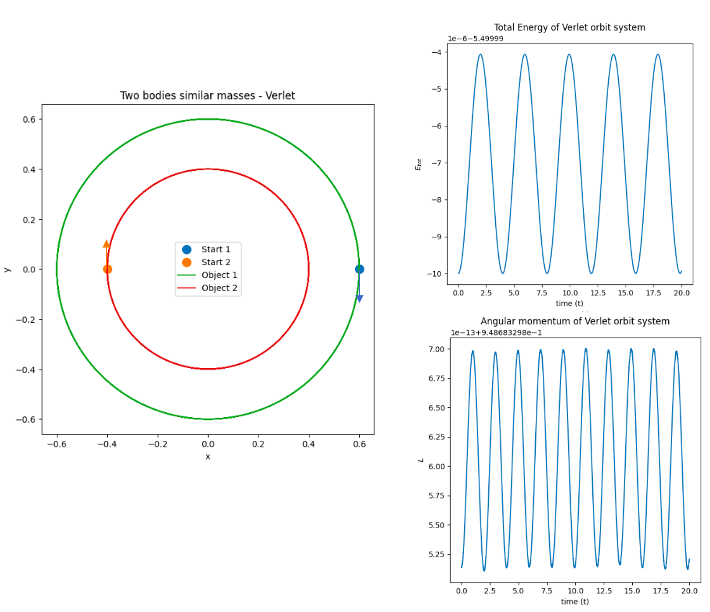
\includegraphics[scale=0.45]{Pictures/Verlet_2bodies.png}}
\caption{Plots from Velocity Verlet 2 body simulation}
\label{2BodyGraph}
\end{figure}



\subsection{Analysis of the graphs}

From these graphs we can clearly see that it is not perfect as we do not get a completely flat line in the energies, instead seeing sinosoidal oscillations. We can see however that the extent of these oscillations are much smaller than with the Euler method. They are on the order of magnitude of 1e-6 compared to 1e-5 for the total energy and 1e-13 compared to 1e-4 for the angular momentum. Looking at the plot of the positions of the objects, we can also see that they don't spiral outwards by any discernible amount.

\subsection{Euler vs Velocity Verlet}

The velocity Verlet method is clearly more accurate than Euler's method, however it does also take more time to calculate the extra terms required in the calculation. The average time taken for the Verlet was more than double that of Euler for my machine. To get any accurate data from the Euler method however, $\Delta t$ does have to be made incredibly small and smaller than its critical value for stability otherwise the method will converge very slowly or never converge at all. 


% --------------------------------------------------SECTION 5---------------------------------------------------------------------------------------------------------------------
\centering
\section{The 3 body problem}
\raggedright

The 3 body problem is still an important problem in physics due to it being impossible to fully solve analytically (though some solutions have been found, most notably by Euler and Lagrange in 1772). We will first look at the three body problem for a Star-Planet-Moon (S-P-M) like orbit. We will be studying this problem using both velocity Verlet as described earlier and a new integrator, the Runge Kutta 4th order.

\subsection{Runge Kutta}

%%%%------- Look up what RK45 method actually does
Runge Kutta 4th order is another explicit differential equation solver, however rather than coding in the algorithm itself, I will be using the SciPy inbuilt python function: integrate.solve\_ivp setting the method to 'RK45'. In the documentation for this solver, it is said: "\textit{The error is controlled assuming accuracy of the fourth-order method, but steps are taken using the fifth-order accurate formula (local extrapolation is done)} \cite{SciPy}. To get the 'RK45' method to work reliably I had to manually set the relative tolerance inside the solver to 1e-6. A lower value could have been used to obtain more accurate results, however this would have increased the computational workload. Manually setting this value ensures the solver never takes too large of a step and keeps errors down, which is useful for complex orbits or orbits where the numbers involved have a large order of magnitude difference. The default value for the relative tolerance is 1e-3. Because of the 4 terms used in the Runge Kutta algorithm, the global error of the algorithm is on the order of $(\Delta t)^4$. \cite{RK45Error}


\subsection{Three bodies in Star-Planet-Moon type orbit}

%%NEED to get energy update cycle going in RK and plot initial positions

We will first be testing these two solvers in a Star-Planet-Moon (S-P-M) type orbit. To do this calculation we will consider the orbit of the centre of mass of the outer bodies (called body 23) around body 1 (close to the origin) and then the orbit of bodies 2 and 3 around their centre of mass. For this problem we will set the masses to 1, 3e-6 and 3.6e-8 for bodies 1, 2 and 3 respectively. We also want to have the starting distance between body 1 and 2 to be 1 and between body 1 and 3 to be 1.0025.

\subsection{Potential Energy calculations}

To calculate the potential energies for this orbit I summed:
\begin{itemize}
 \item The potential energy of body 1 due to body 23
 \item The potential energy of body 2 due to body 3
 \end{itemize}



\subsection{Initial conditions calculations}

We want to place the COM at the origin, with all masses lined up in x direction. This gives us the equations:

$$ 
\frac{m_1 x_1 + m_2 x_2 + m_3 x_3}{m_1 + m_2 + m_3} = 0 
$$
$$
x_2 - x_1 = 1 \Rightarrow x_1 = x_2 - 1 
\newline
$$
$$
x_3 - x_2 = 0.025 \Rightarrow x_3 = 0.025 + x_2
$$
From this we can work out:
$$
x_2 = \frac{1 - m_3 \times 0.025}{1 + m_2 + m_3}
$$
Which means we can work out $x_2, x_3 $ and $  x_{23}$ (the distance between origin and centre of mass of object 2 and 3).

The velocity of mass 1 of these can then be calculated from:

$$ \frac{G m_1 m_{23}}{r_{1->COM}} = \frac{m_1 v_1^2}{r_{1->23}} $$

Where $r_{1->COM}$ is the vector between mass 1 and the centre of mass of the entire system (in this case the origin) and $r_{1->23}$ is the vector between mass 1 and mass 23.

Similarly equations for $v_2, v_{23}$ and $v_3$ can be found.


\subsection{Verlet S-P-M orbit plots}

\begin{figure}[!ht]
\centerline{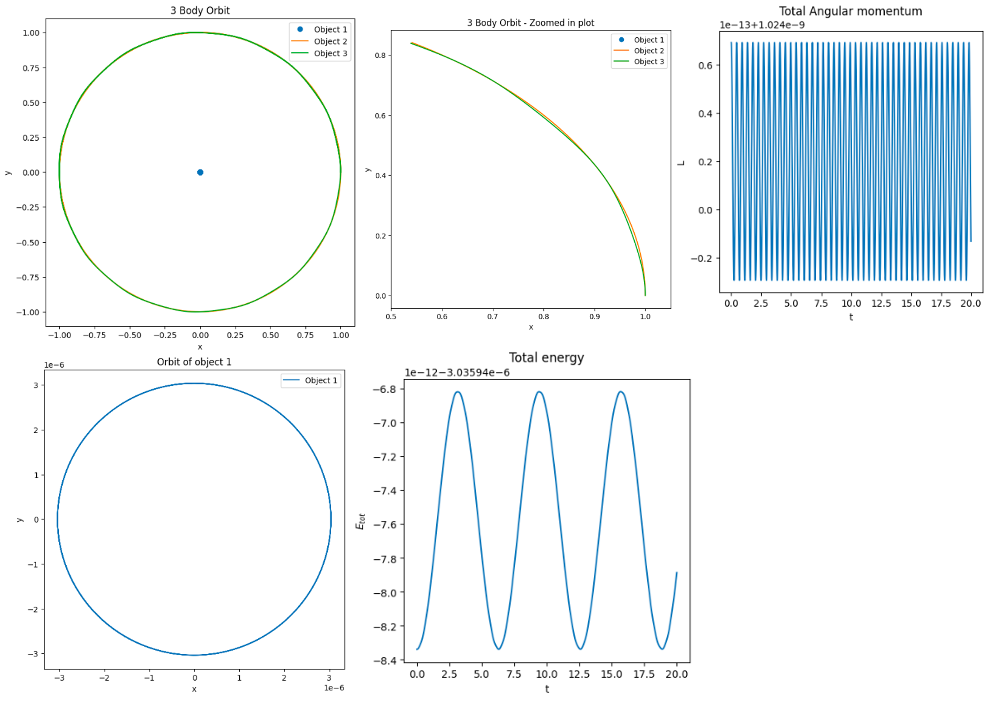
\includegraphics[scale=0.39]{Pictures/SEM_verlet_cor.png}}
\caption{Plots from Velocity Verlet S-P-M orbit}
\label{SEM_verlet}
\end{figure}


\subsection{Analysis of Verlet Plots}

From graph \ref{SEM_verlet}a we can see that body 1 barely moves and bodies 2 and 3 move in a very similar circular orbit around body 1. In the zoomed in graph (fig \ref{SEM_verlet}b) we can see that body 3 does indeed orbit around body 2.
\smallskip

From the graphs of the energy and angular momentum we can see both the energy and angular momentum vary very slightly (on order of 1e-12 and 1e-13) in a sinosoidal pattern. This small variation in energy is expected for velocity Verlet as it is a time reversible method, focused on energy conservation and while we can see the energy is not constant, it does not drift over time and stays in the same sinusoidal pattern throughout the orbit.


\subsection{Runge-Kutta S-P-M orbit plots}


\begin{figure}[!ht]
\centerline{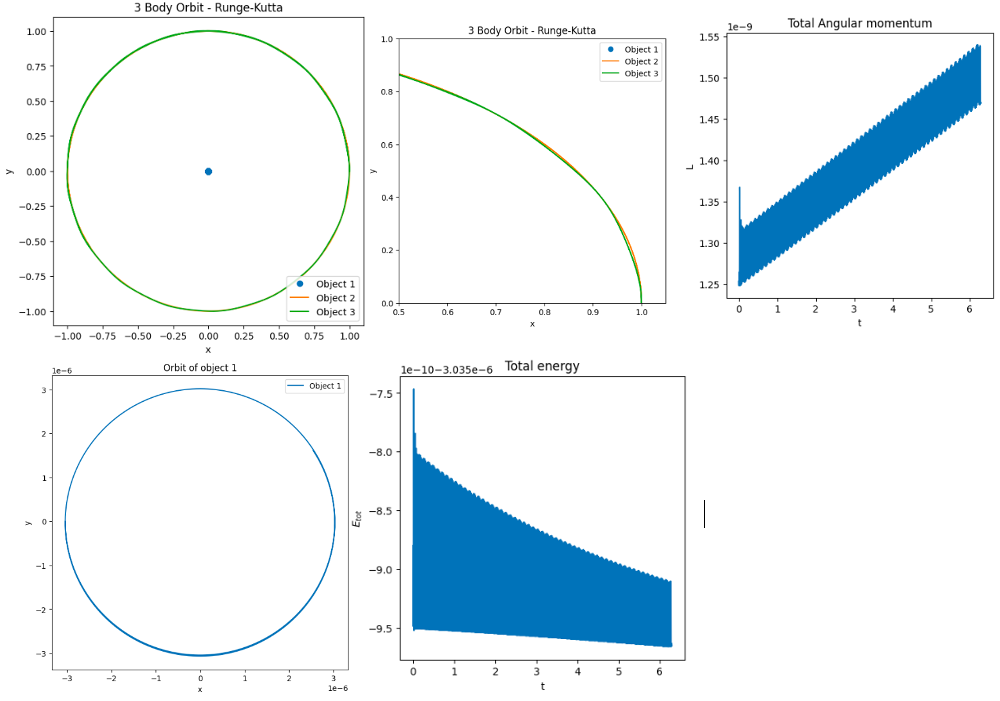
\includegraphics[scale=0.38]{Pictures/SEM_RK.png}}
\caption{Plots from Runge-Kutta S-P-M orbit}
\label{SEM_RK}
\end{figure}


\subsection{Analysis of Runge-Kutta plots}

From graphs \ref{SEM_RK}a, \ref{SEM_RK}b and \ref{SEM_RK}d, the 3 bodies appears to follow a very similar path to velocity Verlet, however the energy and angular momentum graphs look very different despite being calculated in exactly the same way. While the Runge Kutta method has a lower global error, it is not a time reversible algorithm meaning it does not have as much of a focus on energy and angular momentum conservation. The variation on this energy is still very small though - on the order of 1e-10 and 1e-9 for KE and PE respectively. The error in conservation laws found here is to be expected though given the relative tolerance used within the solver was 1e-6, so errors smaller than the tolerance are expected.

\smallskip

We will see below that the motion of body 3 is the same, or at least very similar by looking at the Laplace-Runge-Lenz-Pauli eccentricity vector.

\subsection{Eccentricity of body 3}

We can analyse the eccentricity of a bodies orbit using the Laplace-Runge-Lenz-Pauli vector. This can help us analyse if the two orbits for Verlet and Runge-Kutta produce the same motion for body 3. The Laplace-Runge-Lenz-Pauli vector is calculated from the equation:

$$ L = \frac{\textbf{r}_R}{r_R} - \frac{v_R^2 \textbf{r}_R - (\textbf{r}_R \cdot \textbf{v}_R) \textbf{v}_R}{G(M_E + M_M)} $$

Where a subscript R means the relative earth moon position \cite{Briefing}.
\smallskip

We will plot the x and y components of this value over time for 3 periods.

\begin{figure}[!ht]
\centerline{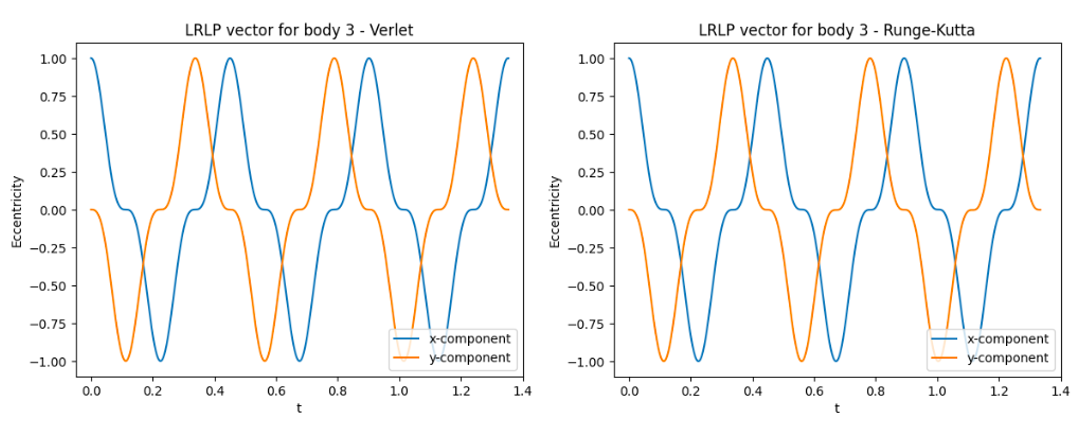
\includegraphics[scale=0.45]{Pictures/SEM_LRLP.png}}
\caption{Laplace-Runge-Lenz-Pauli vector for Verlet and Runge-Kutta methods}
\label{SEM_LRLP}
\end{figure}

\bigskip

It is clear to see that the graph produced for both methods is very similar, with body 3 having the same orbital time period on both. This shows us that while Runge-Kutta may not conserve energy throughout its solution, it still produces an accurate result that agrees with a method that does conserve energy.

\bigskip

For the rest of this paper I will be using the Runge-Kutta method, as it has a lower global error and is easier to implement in code due to it being inbuilt in SciPy.


% --------------------------------------------------SECTION 6---------------------------------------------------------------------------------------------------------------------
\centering
\section{Furthering the 3 body problem}
\raggedright

There are a number of ways to extend the S-P-M like 3 body orbit discussed earlier. One of these which we will now look at is looking for choreographies of 3 or more bodies. N-body choreographies are described as `\textit{a periodic solution to the n-body problem in which all the bodies are equally spread out along a single orbit}' \cite{Choreography}. This paper will look at these solutions for bodies of equal masses (all set to 1).

A specific solution to this problem was first found by Euler and Lagrange in 1772. Their solution is for 3 bodies arranged in an equilateral triangle (known as Lagrange points).

\subsection{Lagrange points and circular orbits}

The solution Euler and Lagrange found for 3 bodies arranged in an equilateral triangle can in fact be generalised to any regular polygon where the bodies are placed at the vertices of the polygon and spun with the same angular frequency. This results in a circular orbit where all bodies follow the same circular path, at the same, constant distance from each other meaning they all move at fixed angular velocity throughout the orbit.

The calculation of the angular frequency gets much more complicated for more than 3 bodies. I used the equation derived in a paper by V\'{i}ctor S\'{a}nchez Li\~{n}\'{a}n \cite{angspeed}:

$$
\lambda = \frac{m}{lr^2}(1+\frac{l}{n}(\sum_{j=3}^{n-1} \frac{1}{r_{1j}} \sum_{i=2}^{n-2} \sum_{j=i+2}^{n} \frac{1}{r_{ij}})
$$
where $l$ is the length of one side of the n-gon and
$$
\omega = \pm \sqrt{\lambda}
$$

Where the $\pm$ just determines whether the rotation is clockwise or anti-clockwise.

\subsection{Plots of circular orbits for 3 to 8 bodies}

\begin{figure}[!ht]
\centerline{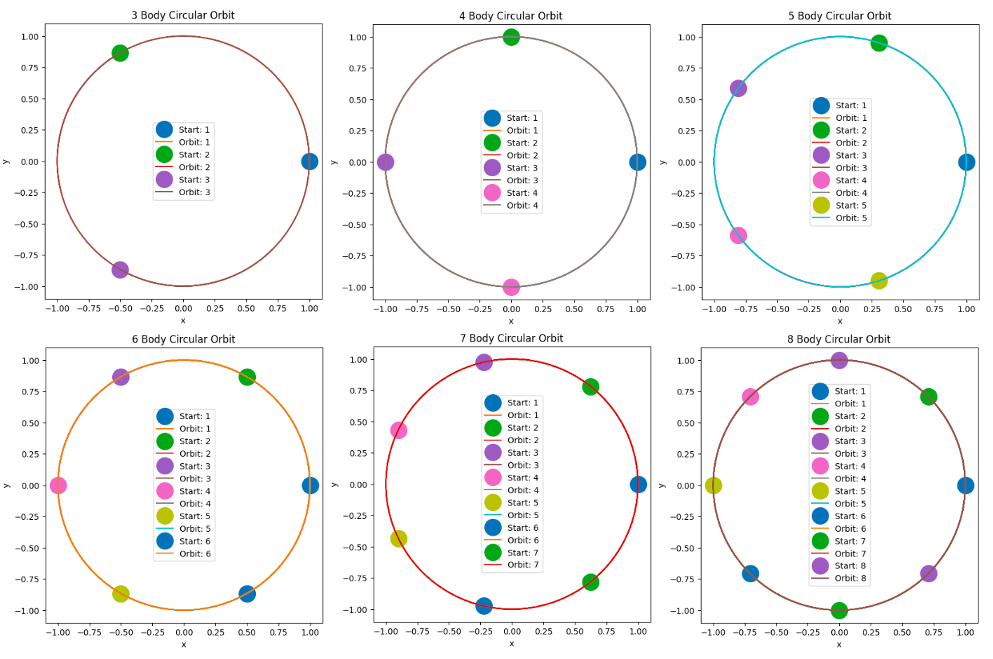
\includegraphics[scale=0.33]{Pictures/Circular_orbits.png}}
\caption{Circular choreographies for 3 to 8 bodies}
\label{Circ_3_8}
\end{figure}


\subsection{Stability of the circular orbits}

The circular orbits found here are stable, but when the number of bodies is increased, there is an increased sensitivity to the precision of initial conditions and precision within the solver used. This can be seen clearly from the plot of the 9 body circular orbit (fig \ref{Circ_9}).


\begin{figure}[!ht]
\centerline{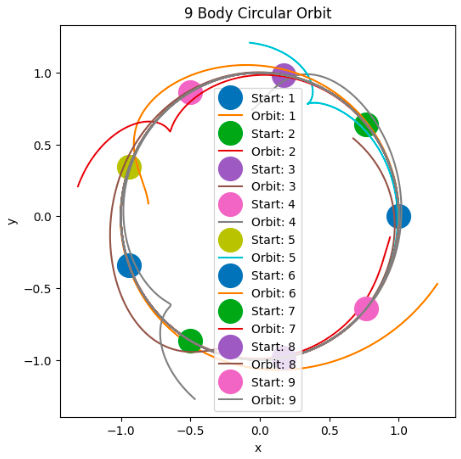
\includegraphics[scale=0.35]{Pictures/9BodyCircular.png}}
\caption{Circular orbit for 9 bodies}
\label{Circ_9}
\end{figure}

This uses the same code and precision as circular orbits 3 through 8, however does not appear to be stable beyond the very start. In fact for all circular orbits, due to machine precision and solver accuracy, the orbits will never be eternally stable. To fix this a smaller time step or a smaller tolerance within the solver could have been used, however it already takes several minutes to simulate 9 bodies, so lowering the time step or tolerance will only make this take longer. The instabilities encountered in the computer simulation is of course not reflective of the real world where we do not encounter the same errors.


\subsection{Linear chain choreography}

There are more n-body choreographies that have be found than just the Lagrange points. One of these is the linear chain (known as the Gerver SuperEight for 4 bodies). In this paper we will be looking at the 4 body and 6 body versions of the linear chain. The initial conditions for the simulation of these is obtained from \cite{NbodyLinearChain} and can be seen below:
\begin{figure}[!ht]
\centerline{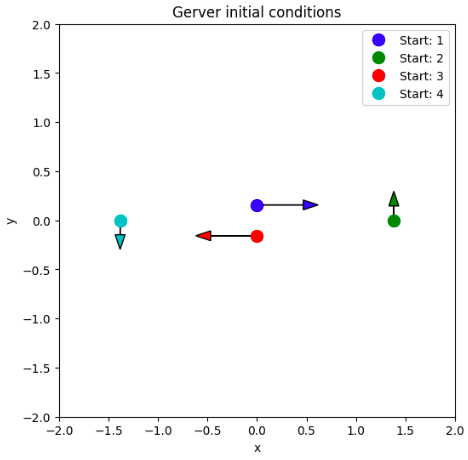
\includegraphics[scale=0.3]{Pictures/Gerver_SuperEight_init.png}}
\caption{Gerver SuperEight initial positions and velocities}
\label{Gerver_SuperEight_init}
\end{figure}


\newpage

\subsection{Plots of Gerver SuperEight}
\begin{figure}[!ht]
\centerline{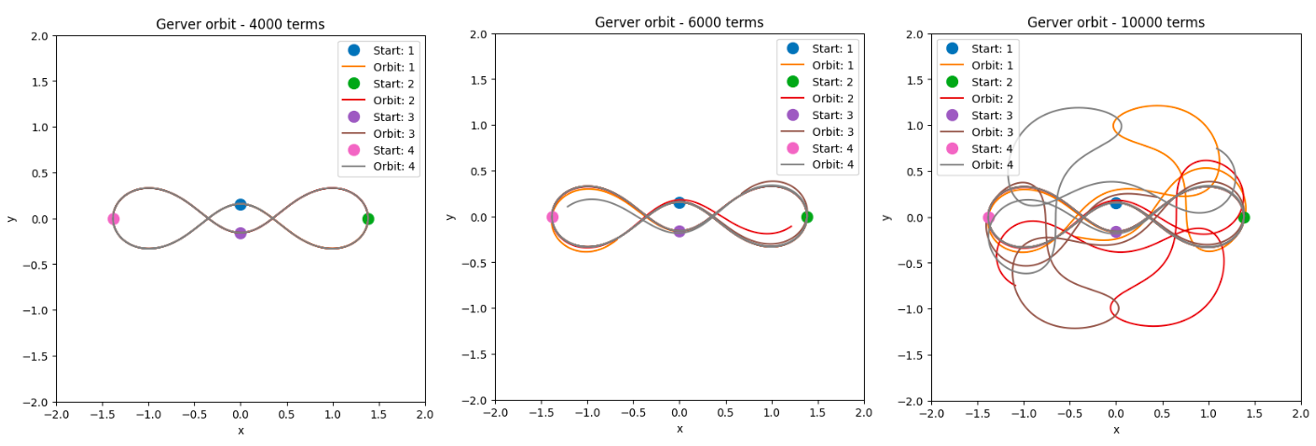
\includegraphics[scale=0.35]{Pictures/Gerver_SuperEight.png}}
\caption{Gerver SuperEight for 4000, 6000 and 10000 terms}
\label{Gerver_SuperEight}
\end{figure}



\subsection{Analaysis of plots of Gerver orbit}

From these plots of the Gerver SuperEight we can see that the bodies do indeed follow a choreography for the first 4000 terms of the simulation, however by 6000 terms they start to deviate from the previous pattern and by 10,000 terms the original shape of the orbit is completely lost and the bodies are no longer following a stable choreography. This does not show that the original orbit is not stable, however instead means that the orbit is very sensitive and does not take much accumulated error over time to deviate from the choreography.


\subsection{Linear chain - 6 bodies plot}


\begin{figure}[ht]
\centerline{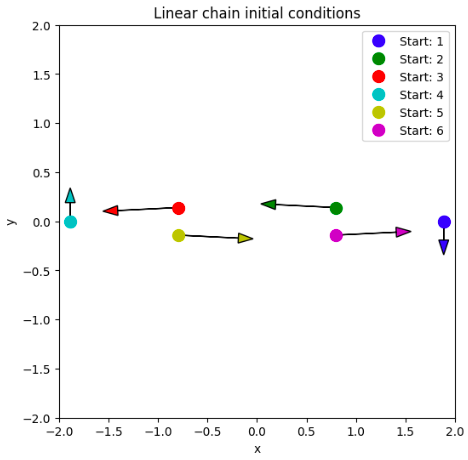
\includegraphics[scale=0.35]{Pictures/LinearChain_init.png}}
\caption{Linear chain initial positions and velocities}
\label{LinearChain_init}
\end{figure}

\begin{figure}[ht]
\centerline{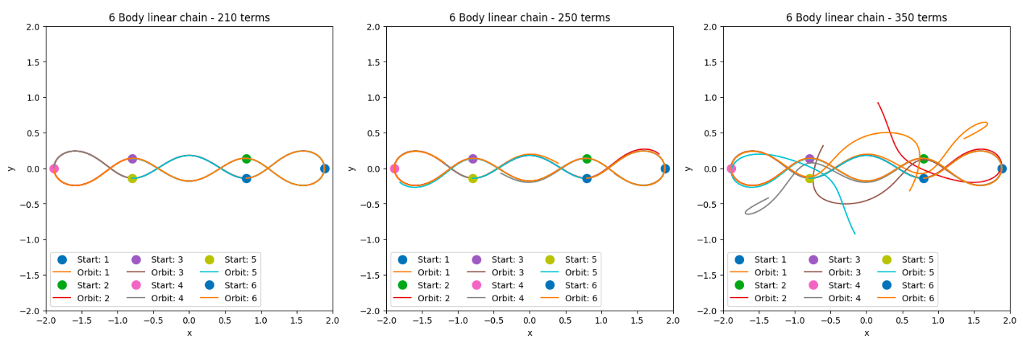
\includegraphics[scale=0.35]{Pictures/LinearChain.png}}
\caption{Linear chain for 210, 250 and 350 terms}
\label{LinearChain}
\end{figure}


\newpage


\subsection{Analysis of linear chain}

From fig \ref{LinearChain} it is clear to see how unstable this orbit is, only appearing stable for the first 210 terms of the orbit and not even after completing a full cycle of the choreography. By 250 terms it has already started visibly differing from the original linear chain and by 350 terms it has lost all stability. This is far less terms (only about 5\%) than for the Gerver SuperEight, therefore is stable for less time in the simulation. This is because there is an extra 2 bodies to simulate for every step which actually more than doubles the number of calculations every step which means errors accumulate faster. Having more bodies also increases the sensitivity to initial conditions as well, similarly to what was seen for the circular orbits in fig \ref{Circ_9}.

% --------------------------------------------------SECTION 7---------------------------------------------------------------------------------------------------------------------
\centering
\section{Complex Choreoographies}
\raggedright

%\newgeometry{left=0.6cm,bottom=0.01cm,top=0.7cm,right=0.6cm}

As well as the simple choreographies found and simulated earlier, complex choreographies of 3 bodies have also been found. A complex choreography is one where bodies have the same mass, but do not follow the same path with a differing phase.
\smallskip

For all of these choreographies we will be using the research presented by Milovan \v{S}uvakov and V. Dmitra\v{s}i- novi\'{c} in their 2013 paper \textit{Three Classes of Newtonian Three-Body Planar Periodic Orbits}. \cite{ComplexNbody}

\smallskip

In this paper they perform: \textit{a numerical search for periodic orbits of three equal masses moving in a plane under the influence of Newtonian gravity, with zero angular momentum} \cite{ComplexNbody}. 
In this report we simulated the orbits found using the initial conditions given in the paper and analysing both their orbits and angular momentum.



To calculate the angular momentum for this system I used the equation:

$$L = m (v \times r)$$

Where $r$ is the distance from the object to the centre of mass. I plotted the z component of the angular momentum rather than its modulus as the orbits are entirely in the x, y plane so the cross product only gives values in the z direction. To get the magnitude of the angular momentum one can just take the absolute value of the angular momentum in the z direction, however this was not done here as it can make it harder to analyse trends in the angular momentum graph.

All orbits are calculated and plotted for 2 time periods of their orbits.
\newgeometry{left=0.6cm,bottom=0.8cm,top=0.8cm,right=1.2cm}

\centering
\subsection{Plots of some complex choreographies and their Angular Momentum}

\begin{figure}[ht]
\begin{tabular}{cccccc}
\subfloat{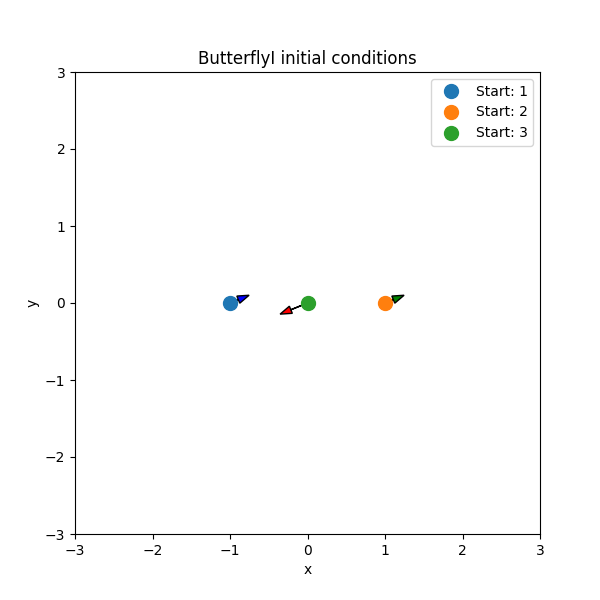
\includegraphics[width = \multi in]{Pictures/CHORS/ButterflyI_init}}&
\subfloat{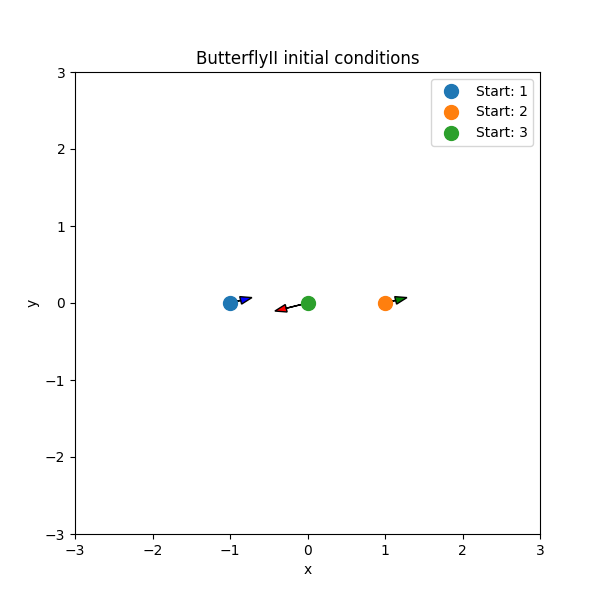
\includegraphics[width = \multi in]{Pictures/CHORS/ButterflyII_init}}&
\subfloat{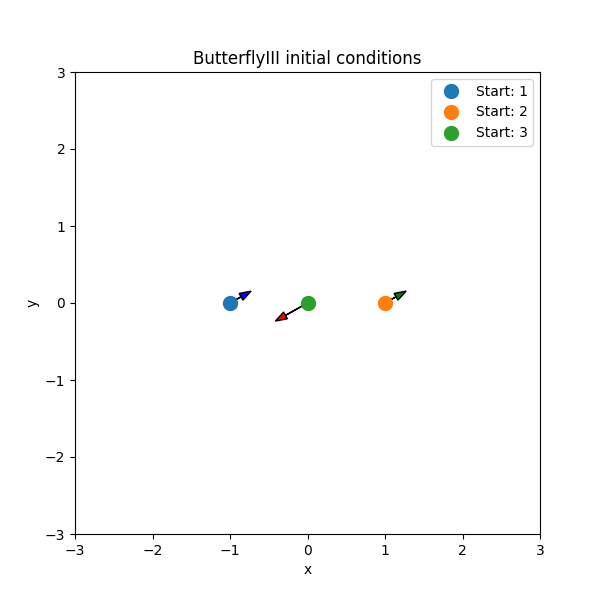
\includegraphics[width = \multi in]{Pictures/CHORS/ButterflyIII_init}}&
\subfloat{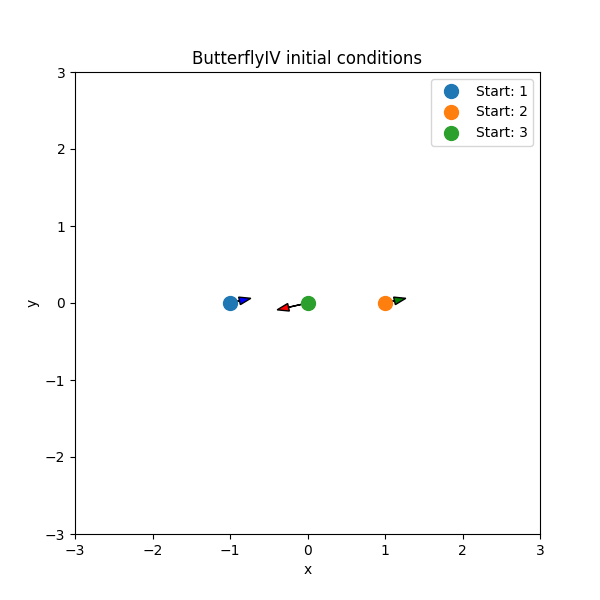
\includegraphics[width = \multi in]{Pictures/CHORS/ButterflyIV_init}}&
\subfloat{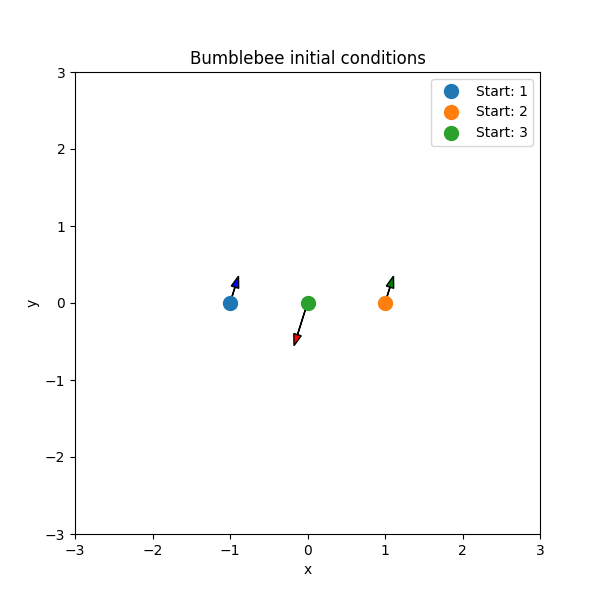
\includegraphics[width = \multi in]{Pictures/CHORS/Bumblebee_init}}&
\subfloat{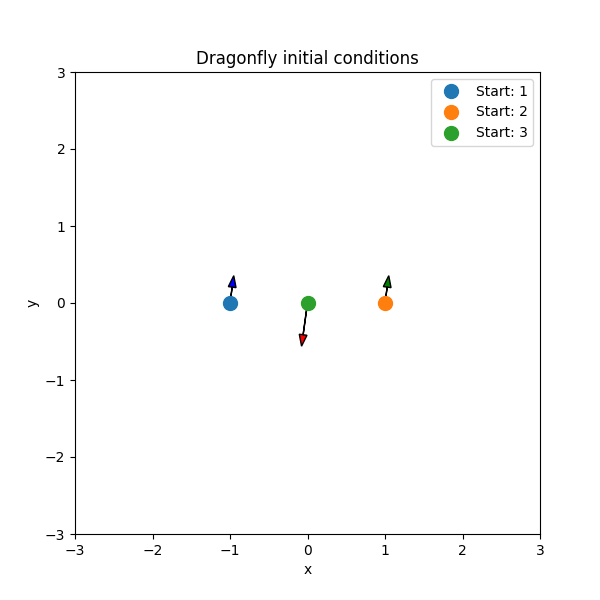
\includegraphics[width = \multi in]{Pictures/CHORS/Dragonfly_init}} \\

\subfloat{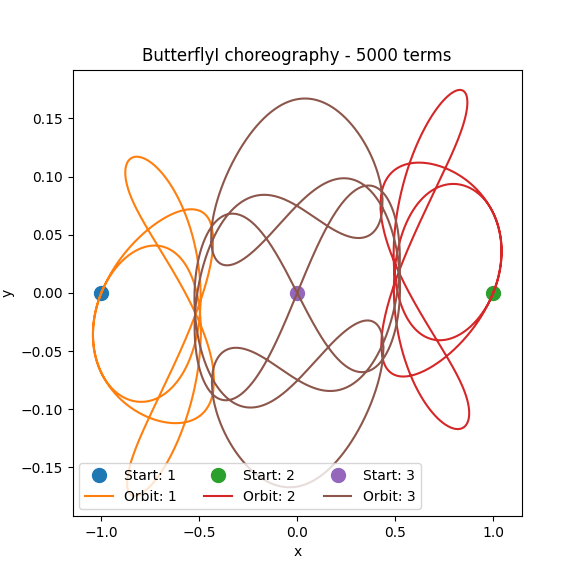
\includegraphics[width = \multi in]{Pictures/CHORS/ButterflyI_final}}&
\subfloat{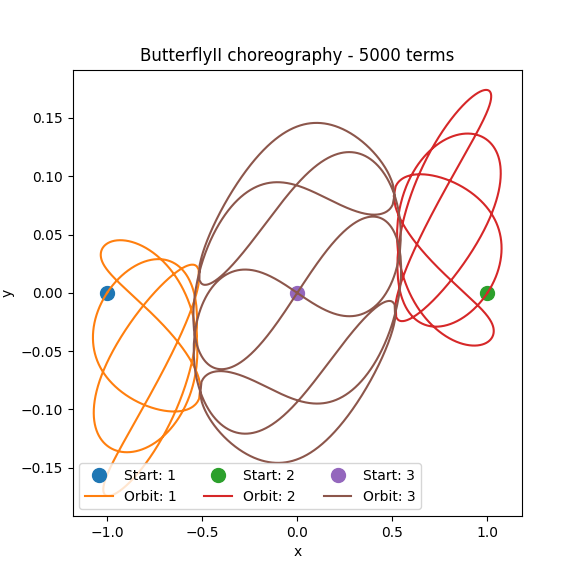
\includegraphics[width = \multi in]{Pictures/CHORS/ButterflyII_final}}&
\subfloat{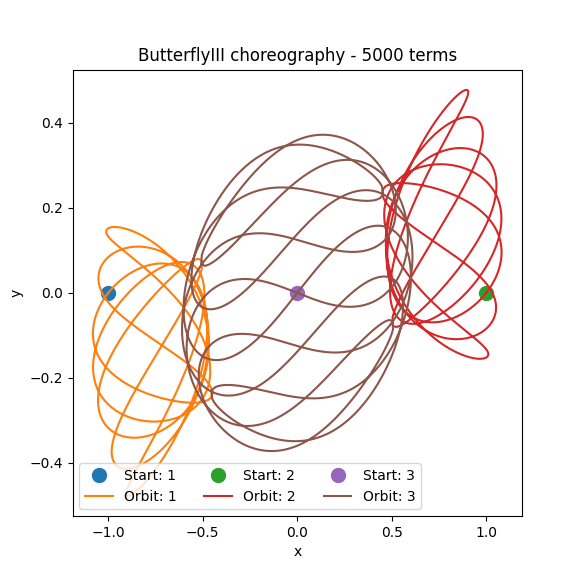
\includegraphics[width = \multi in]{Pictures/CHORS/ButterflyIII_final}}&
\subfloat{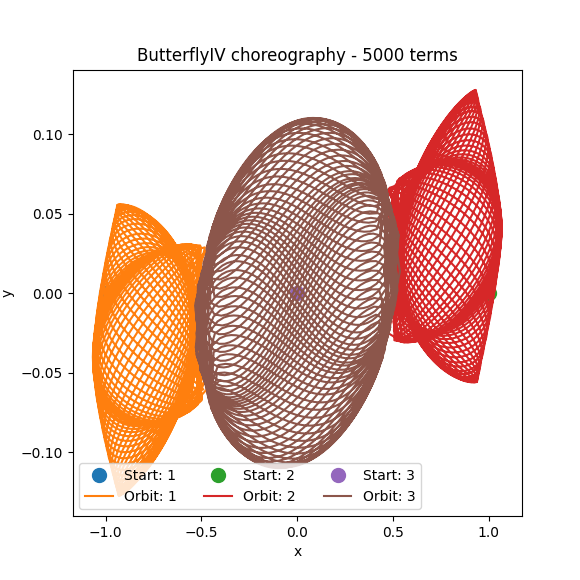
\includegraphics[width = \multi in]{Pictures/CHORS/ButterflyIV_final}}&
\subfloat{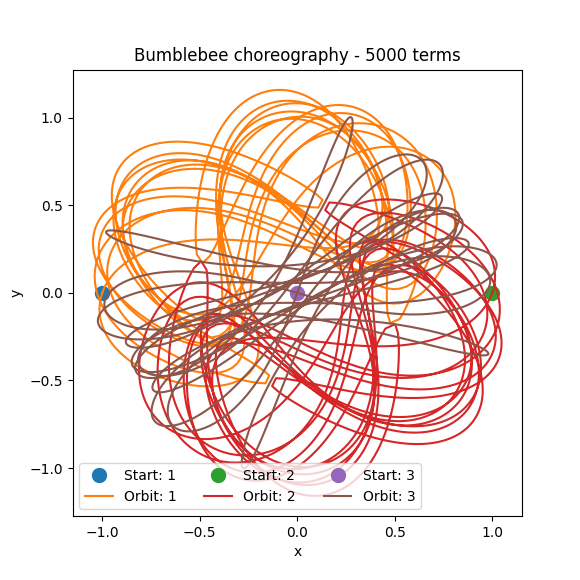
\includegraphics[width = \multi in]{Pictures/CHORS/Bumblebee_final}}&
\subfloat{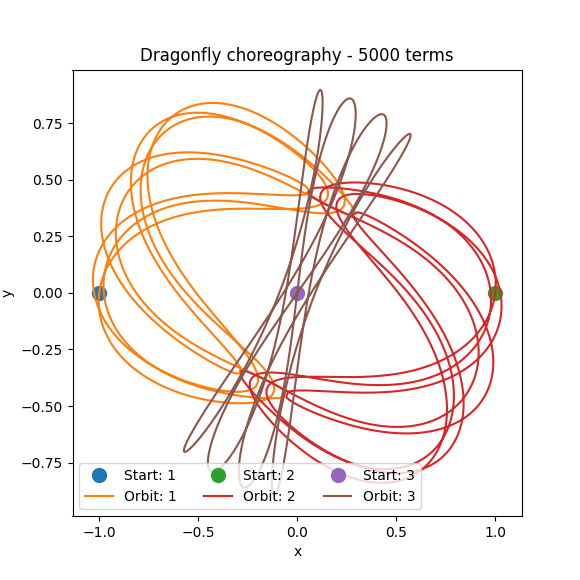
\includegraphics[width = \multi in]{Pictures/CHORS/Dragonfly_final}}\\

\subfloat{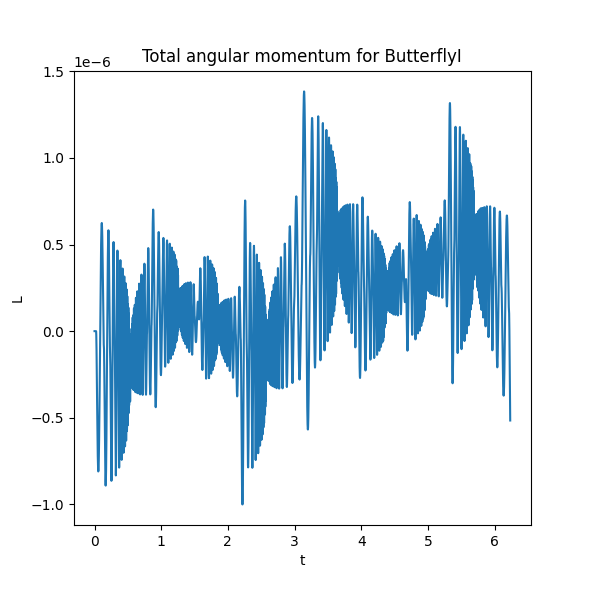
\includegraphics[width = \multi in]{Pictures/CHORS/ButterflyI_angMom}}&
\subfloat{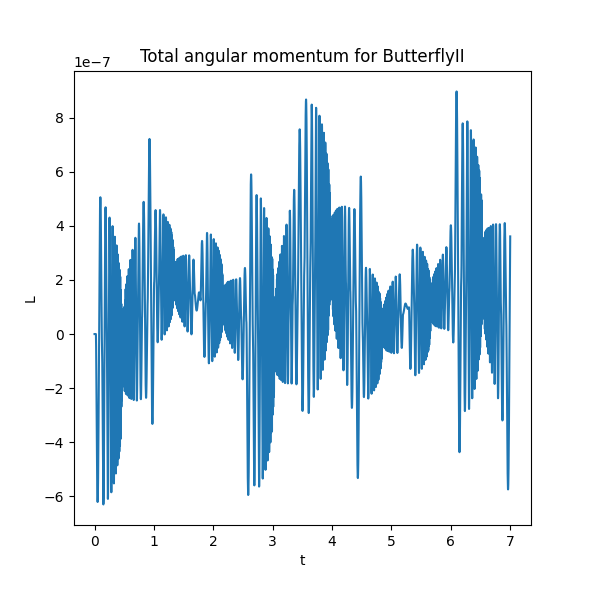
\includegraphics[width = \multi in]{Pictures/CHORS/ButterflyII_angMom}}&
\subfloat{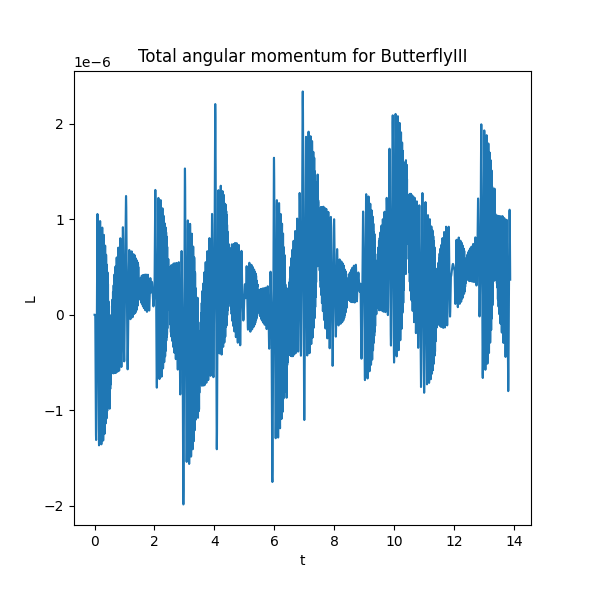
\includegraphics[width = \multi in]{Pictures/CHORS/ButterflyIII_angMom}}&
\subfloat{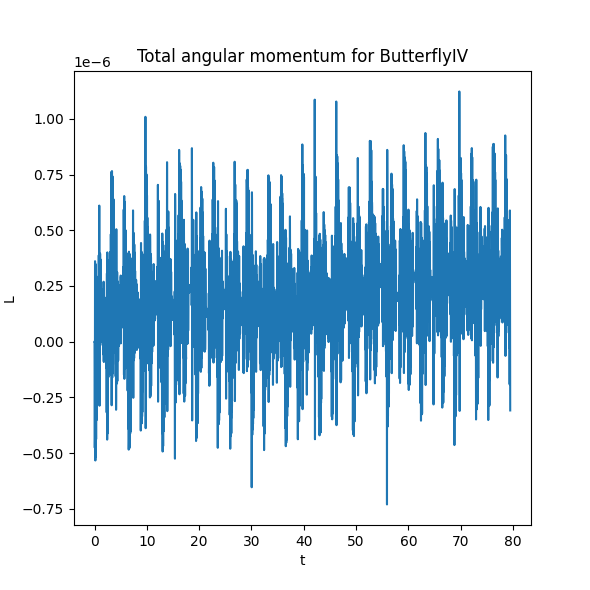
\includegraphics[width = \multi in]{Pictures/CHORS/ButterflyIV_angMom}}&
\subfloat{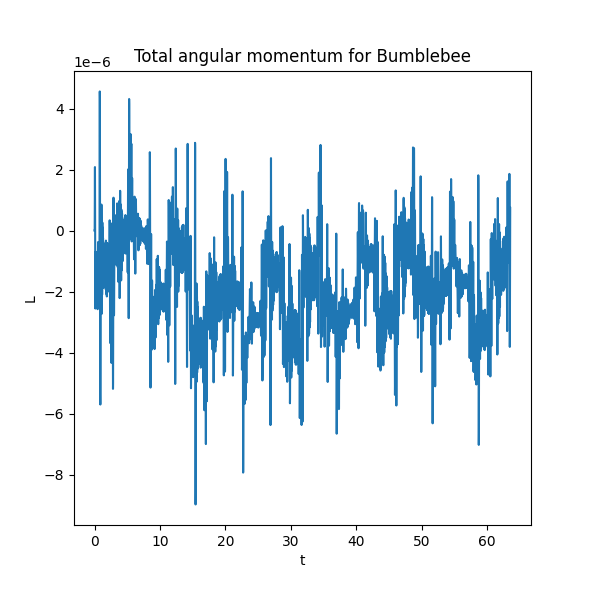
\includegraphics[width = \multi in]{Pictures/CHORS/Bumblebee_angMom}}&
\subfloat{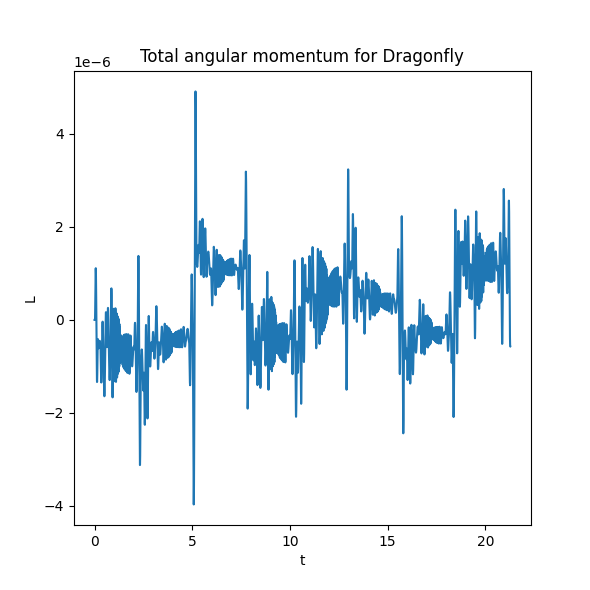
\includegraphics[width = \multi in]{Pictures/CHORS/Dragonfly_angMom}}\\

\subfloat{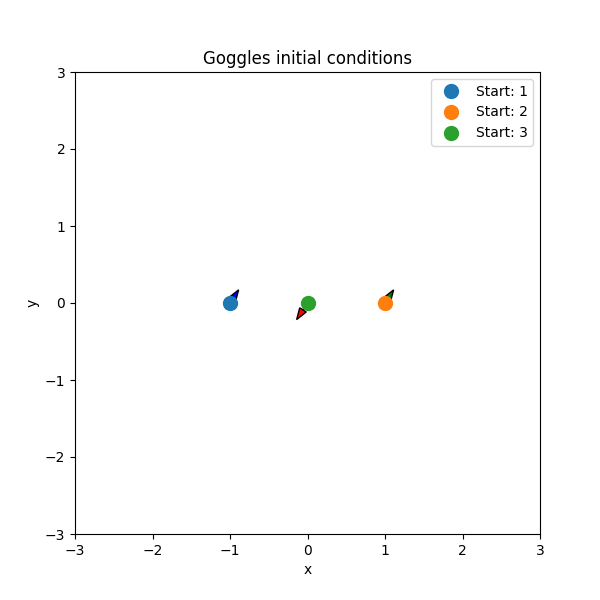
\includegraphics[width = \multi in]{Pictures/CHORS/Goggles_init}} &
\subfloat{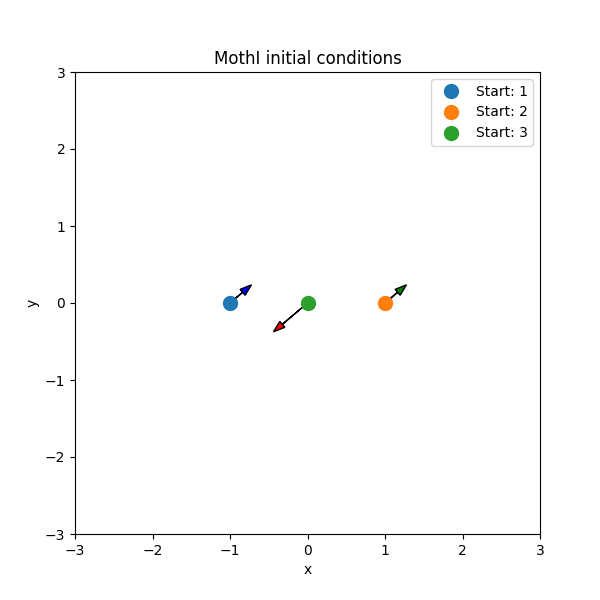
\includegraphics[width = \multi in]{Pictures/CHORS/MothI_init}} &
\subfloat{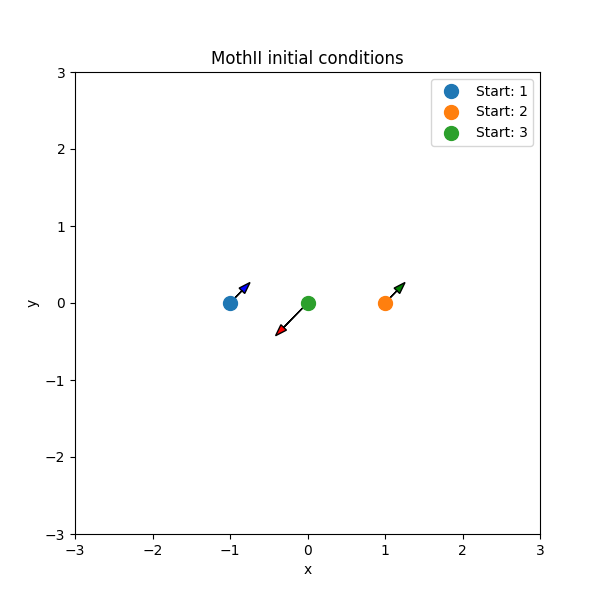
\includegraphics[width = \multi in]{Pictures/CHORS/MothII_init}} &
\subfloat{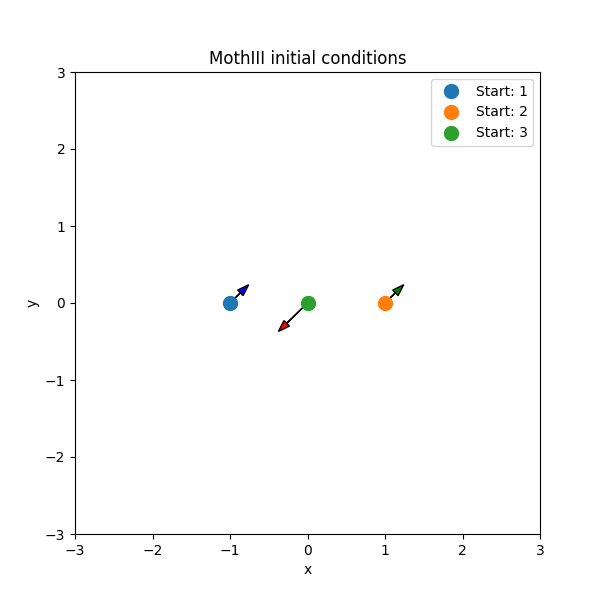
\includegraphics[width = \multi in]{Pictures/CHORS/MothIII_init}} &
\subfloat{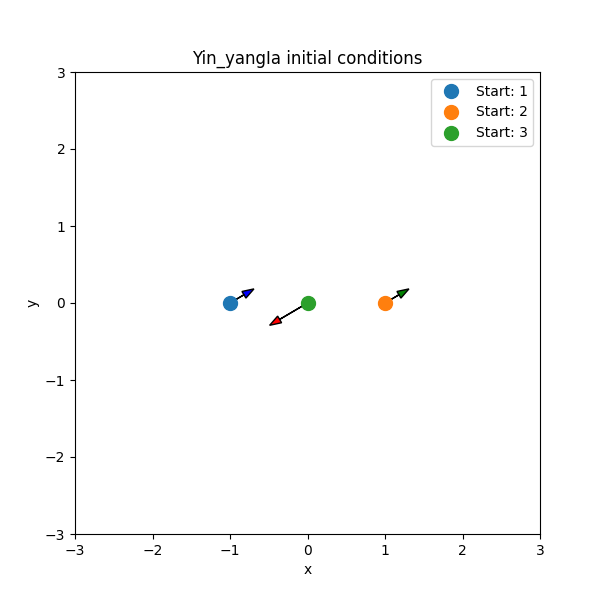
\includegraphics[width = \multi in]{Pictures/CHORS/Yin_yangIa_init}}&
\subfloat{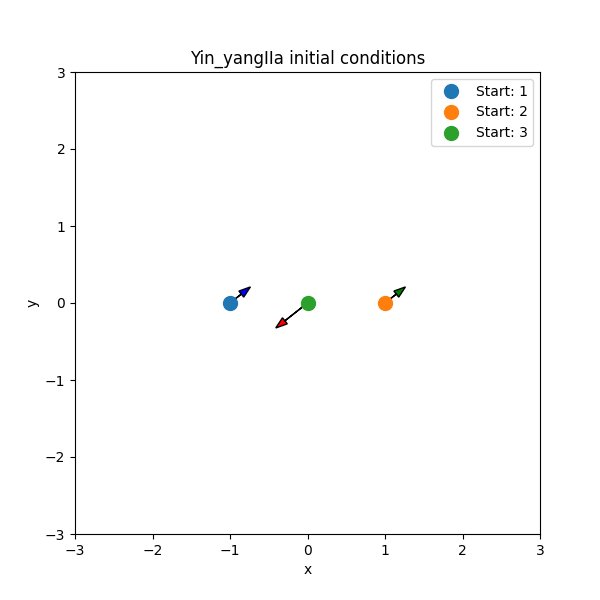
\includegraphics[width = \multi in]{Pictures/CHORS/Yin_yangIIa_init}}\\

\subfloat{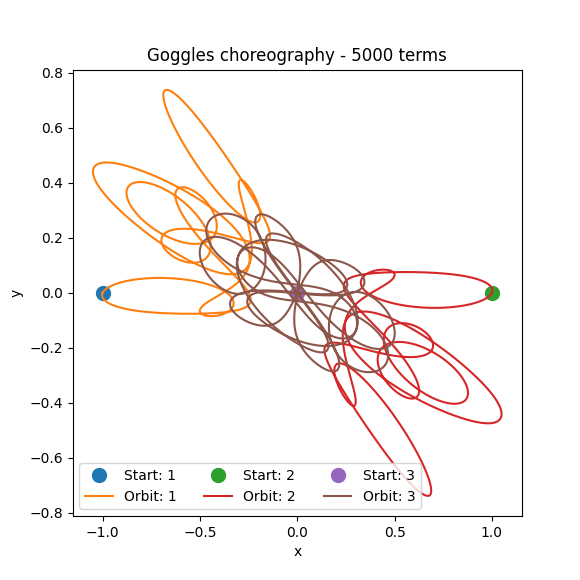
\includegraphics[width = \multi in]{Pictures/CHORS/Goggles_final}}&
\subfloat{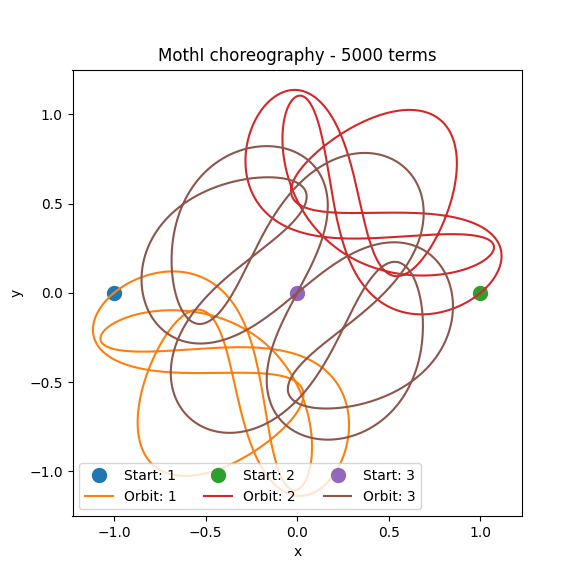
\includegraphics[width = \multi in]{Pictures/CHORS/MothI_final}}&
\subfloat{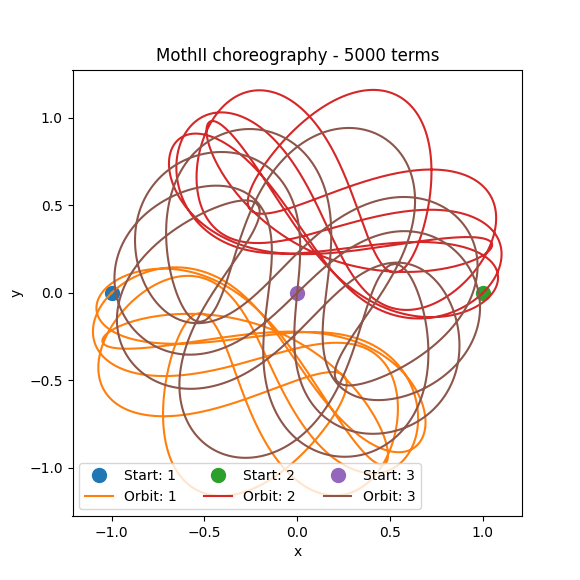
\includegraphics[width = \multi in]{Pictures/CHORS/MothII_final}}&
\subfloat{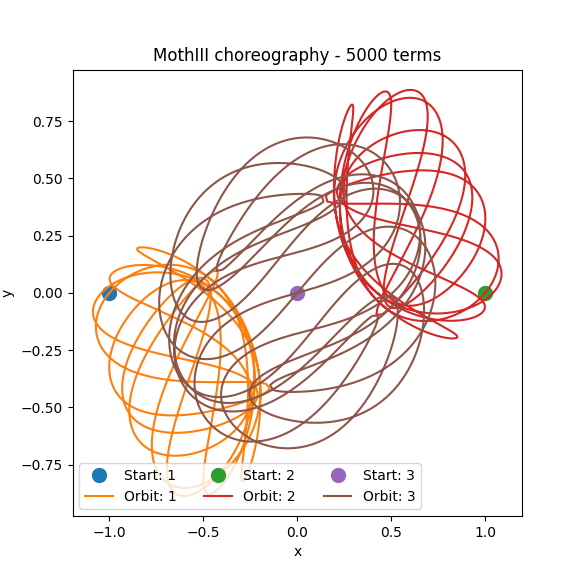
\includegraphics[width = \multi in]{Pictures/CHORS/MothIII_final}}&
\subfloat{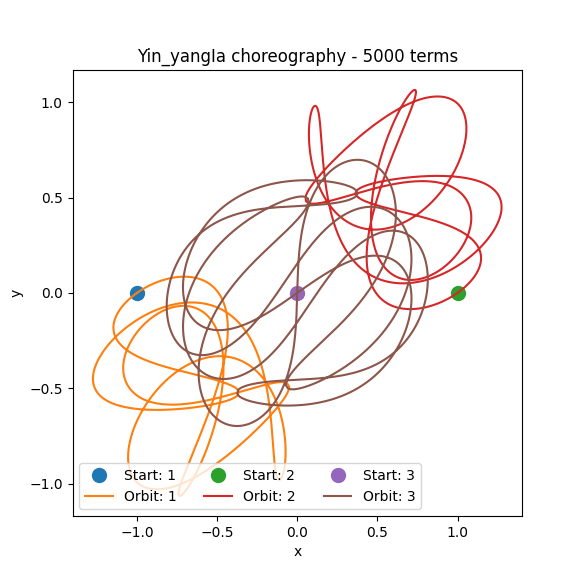
\includegraphics[width = \multi in]{Pictures/CHORS/Yin_yangIa_final}}&
\subfloat{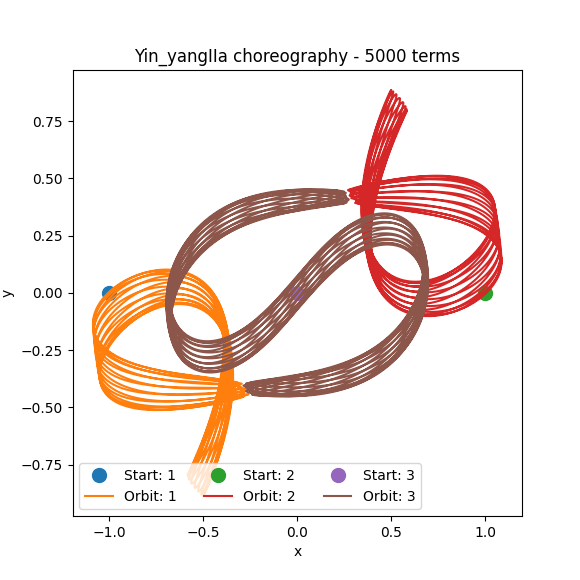
\includegraphics[width = \multi in]{Pictures/CHORS/Yin_yangIIa_final}}\\

\subfloat{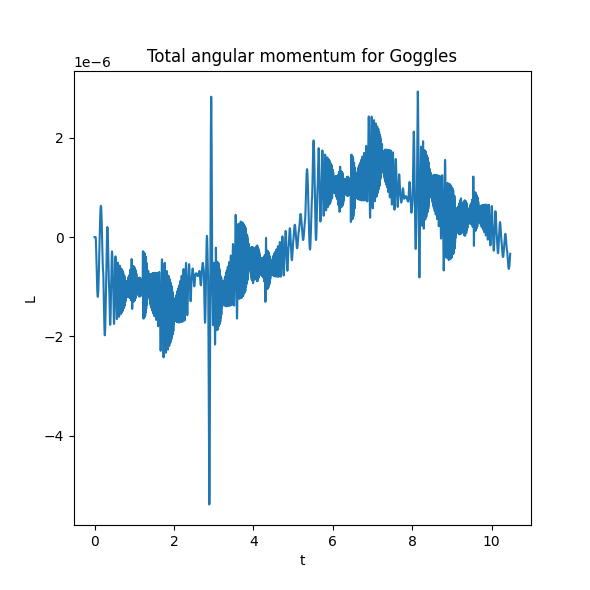
\includegraphics[width = \multi in]{Pictures/CHORS/Goggles_angMom}}&
\subfloat{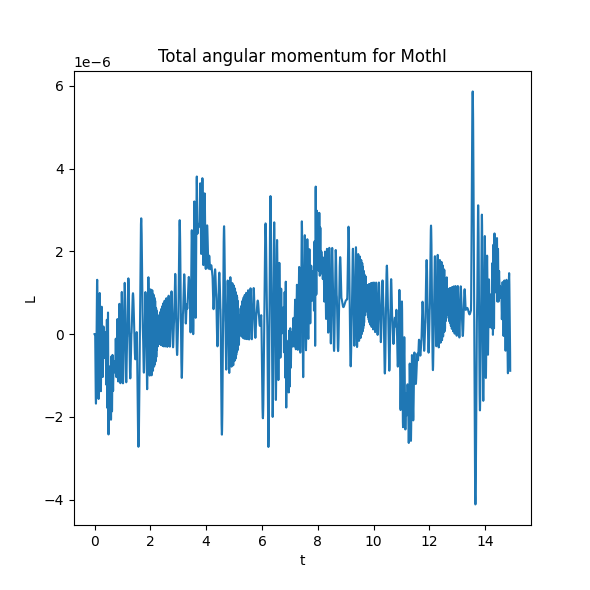
\includegraphics[width = \multi in]{Pictures/CHORS/MothI_angMom}}&
\subfloat{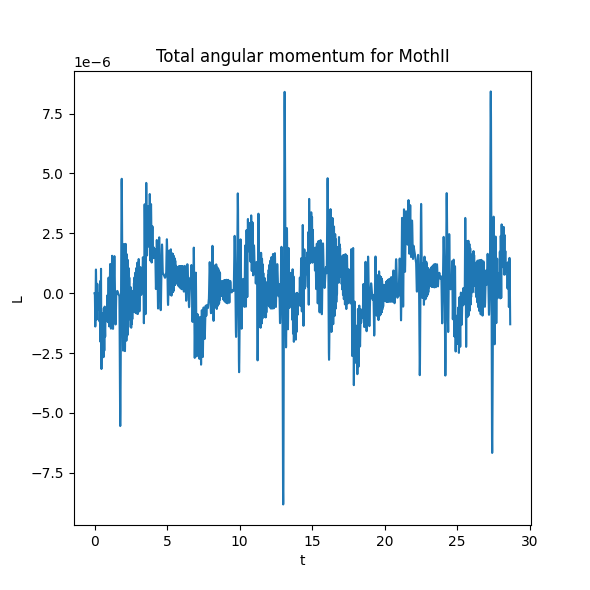
\includegraphics[width = \multi in]{Pictures/CHORS/MothII_angMom}}&
\subfloat{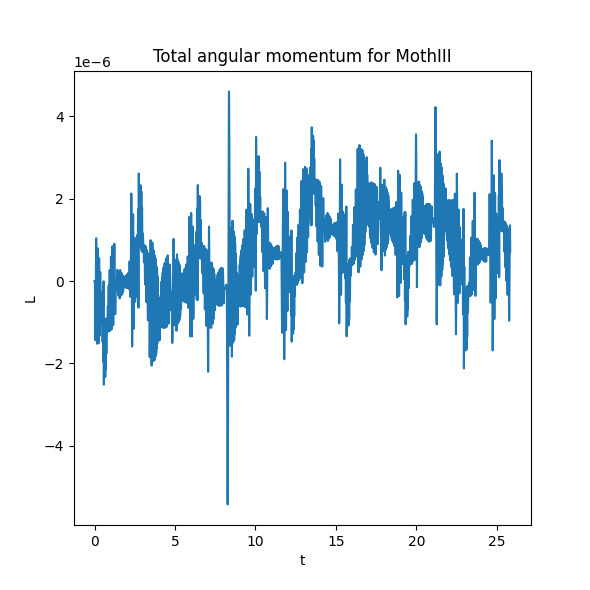
\includegraphics[width = \multi in]{Pictures/CHORS/MothIII_angMom}}&
\subfloat{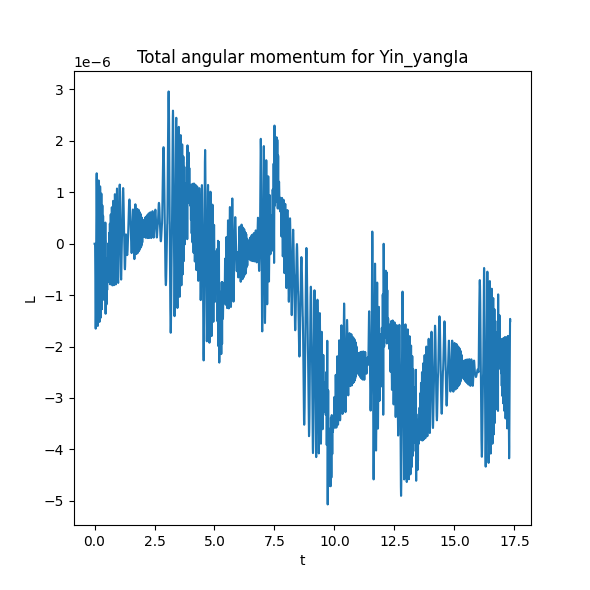
\includegraphics[width = \multi in]{Pictures/CHORS/Yin_yangIa_angMom}}&
\subfloat{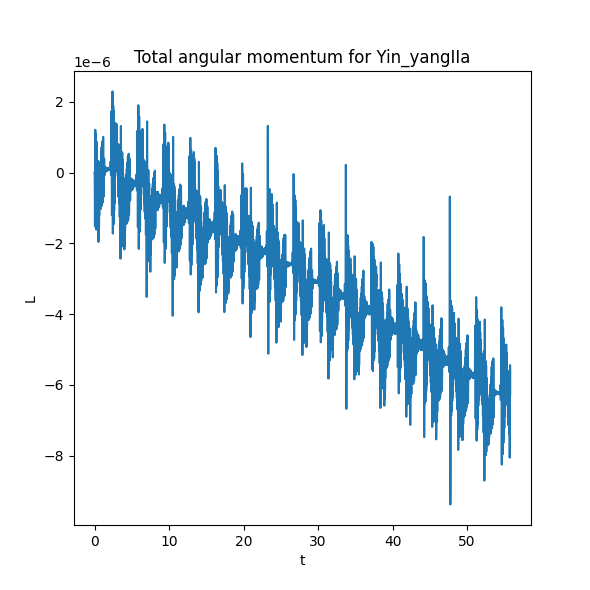
\includegraphics[width = \multi in]{Pictures/CHORS/Yin_yangIIa_angMom}}\\

\end{tabular}
\caption{Complex choreographies of 3 bodies}
\end{figure} 

\restoregeometry
\raggedright

\subsection{Analysis of the complex choreographies}


From these plots of the complex choreographies we can see that the bodies follow some interesting patterns, however taking a closer look at the angular momentum we can see that nearly all the choreographies presented here oscillate around 0 on the order of 1e-6. They are not quite a flat line at 0 because of machine errors and simulation inaccuracies, particularly in the more complex patterns for example Yin\_yang IIa where the angular momentum trends downwards rather than oscillating around 0. For this particular orbit, the increased machine error is likely due to the fast movement of the bodies when they get close together. The speed at which the bodies will be moving at these section will likely mean some of the detail and calculations of the orbit are incorrect due to the time step being too large for the speed of the bodies.


% --------------------------------------------------SECTION 8---------------------------------------------------------------------------------------------------------------------
\centering
\section{Possible improvements}
\raggedright

Possible improvements to the modelling and simulation of the bodies discussed in this paper are as follows. The differential equation solver methods could be upgraded to ones with higher than $(\Delta t)^4$ global error, for example DOP853 from scipy's in built functions. This does, however, have the consequence of adding more calculation terms at each step and the scaling of the algorithms used for higher than fourth order is less good.

\smallskip 

For fourth order and under, the time complexity scales linearly with the power of the error, however for powers of error greater than 6, while it is theoretically possible to have the complexity only scale with power + 1, no algorithm which performs as well as this has been found. For example when the error is of order 7 the number of steps = 9 and when the error is of order 8 the number of steps = 11. We could also have set lower tolerances within the solver, so that it tries to keep the errors within itself down. However, the solver does not always manage to keep the errors within these tolerances and the orbits eventually diverge anyway if simulated for long enough. I settled on a relative tolerance of 1e-6 as it keeps a good balance of not taking too long while keeping stable enough to analyse the orbits.

\medskip

To improve the errors in the differential equation solver methods we could instead reduce the problem to being able to be solved by a zero finding algorithm using the interval Newton method and Krawczyk method as is done in \cite{NbodyLinearChain}. This would also give us more rigorous bounds on the problem as well as being more accurate.



% --------------------------------------------------SECTION 9---------------------------------------------------------------------------------------------------------------------
\centering
\section{Future exploration}
\raggedright

There are many open questions still associated with the choreographies studied in this paper as very little is known about them mathematically due to the lack of an analytic solution for their orbits. One such example of these problems is the uniqueness of the choreographies. We could also explore further by searching for new choreographies that have not yet been found and analysing these.

When simulating more real world situations as well, we could also simulate elliptical orbits rather than circular ones, as these are more realistic to the orbits we observe in our own universe and we have also completely neglected any gravitational relativistic effects on the orbits by working in a Newtonian regime.

More analysis on the period of the choreographies and how exactly they return to their original orbit after a full period (especially for the complex choreographies) could also be done.





% --------------------------------------------------SECTION 10---------------------------------------------------------------------------------------------------------------------
\centering
\section{Conclusion}
\raggedright

During this paper we have looked at both more realistic situations and analysed different solver methods on them, and more theoretical choreographies which we analysed for their stability and existence. For the first of these, we showed that Euler's method has large inaccuracies and large errors in conserved quantities. We also showed that because velocity Verlet is time reversible it has more of a focus on energy conservation as opposed to the Runge Kutta fourth order method, however does have larger global errors.

\smallskip

When looking at regular choreographies we could see that the more bodies were added, the more sensitive the system was to both initial conditions and the global errors accumulated by the solver, loosing almost all stability for 9 bodies in the circular orbit and 6 bodies in the linear chain. For the complex choreographies we could see that the angular momentum of all choreographies found in paper \cite{ComplexNbody} which were claimed to have 0 angular momentum are indeed close to having 0 angular momentum within the errors of the solver used for the simulation (All variations at or below 1e-6).





% --------------------------------------------------SECTION 11---------------------------------------------------------------------------------------------------------------------




\newpage
%%BIBLIOGRAHY


\begin{thebibliography}{9}

\bibitem{NbodyScipy}
Modelling the Three Body Problem in Classical Mechanics using Python - Gaurav Deshmukh
https://towardsdatascience.com/modelling-the-three-body-problem-in-classical-mechanics-using-python-9dc270ad7767



\bibitem{ComplexNbody}
Milovan \v{S}uvakov and V. Dmitra\v{s}i- novi\'{c}. Three Classes of Newtonian Three-Body Planar Periodic Orbits. Phys. Rev. Lett., 110:114301, 2013
https://journals.aps.org/prl/abstract/10.1103/PhysRevLett.110.114301

\bibitem{NbodyLinearChain}
Tomasz Kapela and Piotr Zgliczy\'{n}ski. The existence of simple choreographies for the N-body problem—a computer- assisted proof. Nonlinearity, 16:1899, 2003

\bibitem{Briefing}
PHAS0030: Computational Physics Mini-project briefing: complex orbital dynamics David Bowler
February 17, 2023

\bibitem{angspeed}
Special Solutions of the N-Body Problem: Central Configurations and Choreographies - V\'{i}ctor S\'{a}nchez Li\~{n}\'{a}n
https://diposit.ub.edu/dspace/bitstream/2445/181716/2/tfg\_victor\_sanchez\_linan.pdf

\bibitem{SciPy}
SciPy Documentation for solve\_ivp.
https://docs.scipy.org/doc/scipy/reference/generated/scipy.integrate.solve\_ivp.html

\bibitem{RK45Error}
Fourth order Runge-Kutta Erik Cheever
https://lpsa.swarthmore.edu/NumInt/NumIntFourth.html

\bibitem{Choreography}
Vanderbei, Robert J. (2004). "New Orbits for the n-Body Problem". Annals of the New York Academy of Sciences. 1017 (1): 422–433. arXiv:astro-ph/0303153. Bibcode:2004NYASA1017..422V. CiteSeerX 10.1.1.140.6108. doi:10.1196/annals.1311.024. PMID 15220160. S2CID 8202325.

\bibitem{Errors}
J. C. Butcher, Runge–Kutta Methods in Modern Computation, Part I: Fundamental Concepts
https://aip.scitation.org/doi/pdf/10.1063/1.168500



\end{thebibliography}



\end{document}